    \documentclass[tcc]{ic}

\hypersetup{
    colorlinks = {true},
    linktocpage = {false},
    plainpages = {false},
    linkcolor = {Blue},
    citecolor = {Blue},
    urlcolor = {Red},
    unicode = {true},
    pdftitle = {Alexis Rapport des enseignements à l'IUT UPPA du 22-01-2024 au 08-02-2024}, 
    pdfauthor = {Alexis Déhu},
    pdfsubject = {Rapport de mes enseignements reçus à l'IUT de Mont-de-Marsan pour la troisième période de ma deuxième année de BUT R&T du 22-01-2024 au 08-02-2024},
    pdfkeywords = {enseignements, apprentissage, alternance, iut, but, rt, uppa, pau, mont, de, marsan, mont-de-marsan}
}

\usepackage{algorithm}
\usepackage{algpseudocode}
\usepackage[graphicx]{realboxes}

\makeatletter
\renewcommand{\ALG@name}{Algoritmo}
\renewcommand{\listalgorithmname}{List of \ALG@name s}
\makeatother

\newcolumntype{Y}{>{\centering\arraybackslash}X}

\begin{document}

    % Inclui o preâmbulo do documento (Informações da capa e contracapa)
    \titulo{Rapport des enseignements à l’IUT}

\autor{Alexis Déhu}{a.dehu@aditu.fr}{}


\orientador{M. Angel Abénia}{abenia@univ-pau.fr}{}{}{}
%\examinador{Mr. Guillaume Devesa}{g.devesa@aditu.fr}{}{}{}

\dataMesAno{Septembre}{2023}{}

    \selectlanguage{english}
    
    % Capa, contracapa e avaliadores
    \capa

    % \aprovacao
    
    % Agradecimentos
    % \begin{agradecimentos}

Obrigado

\end{agradecimentos}
    
    % Resumo e Abstract
    \begin{resumo}

    Cette deuxième période la plus longue d'enseignements à l'IUT (5 semaines) nous a permis d'aborder un vaste champ de compétences extrêmement utiles et intéressantes selon moi.
    \\ \\
    Nous avons couvert trois modules de notre parcours cybersécurité orienté vers la sécurisation du service DNS avec DNSsec, de la compréhension des attaques utilisées sur des protocoles répandus dans les réseaux locaux d'entreprises et de la compréhension des technologies et pratiques de chiffrement de nos données.
    \\
    Nous avons aussi aussi à manipuler et intégrer des pare-feux physiques dans un réseau local d'entreprise selon leur besoins.
    \\ \\
    Aspect télécommunications, nous avons abordés les réseaux cellulaires 2G, 3G, 4G et d'autres en profondeur, en parallèle avec l'étude physique et mathématique de moyens transmissions modernes d'émission-réception.
    \\ \\
    Un module intéressant était aussi consacré à l'automatisation de nos tâches d'administrations des systèmes et des réseaux. En complément de l'apprentissage d'un anglais professionnalisé et d'un travail sur notre communication.
    
    \palavrasChave{sécurisation; protocoles; ARP; ICMP; DNS; chiffrement; cryptographie; clés; chiffrement symétrique; chiffrement asymétrique; intégrité des données; confidentialité; authentification; authenticité; signature; certificat; fonctions mathématiques et algorithmiques; OFDM; COFDM; MIMO; CDMA; TDMA; FHSS; féseaux cellulaire; filtres numériques; filtres analogiques}
\end{resumo}
    %% \begin{abstract}
%     Lorem ipsum dolor sit amet, consectetur adipiscing elit. Duis elit tellus, vehicula in justo eget, fermentum aliquet nisi. In id quam mauris. Sed id vehicula libero. Quisque id tortor placerat, consequat ex sed, placerat ante. Ut dui nunc, placerat volutpat ipsum sit amet, dictum pellentesque lacus. Donec leo sem, dictum quis lacus at, ultricies sagittis elit. Mauris sit amet tortor efficitur, luctus justo sit amet, tincidunt tellus. Donec vulputate non risus at tincidunt. Sed accumsan at erat in aliquet. Sed consequat gravida bibendum. Sed fermentum metus sed ex lacinia mattis. Phasellus vel enim nisl. Proin tortor dui, luctus in erat a, dapibus convallis turpis. Maecenas vitae vulputate neque.

%     Etiam ac ante a lorem consectetur varius. Donec vitae dui porttitor, efficitur ante sed, aliquet lectus. Etiam aliquet mattis sagittis. Integer accumsan, est nec vehicula suscipit, nibh nisl varius ante, at convallis urna est dapibus massa. Orci varius natoque penatibus et magnis dis parturient montes, nascetur ridiculus mus. Praesent tempus dolor sit amet metus eleifend porta. Vestibulum eget viverra nulla. Mauris ac condimentum augue, quis molestie tortor. Duis ac condimentum tortor, sed ullamcorper nunc. Vivamus et suscipit arcu. Duis eget rutrum est, sed pellentesque leo. Nulla lorem lacus, faucibus vitae lectus eu, porttitor efficitur ante. Sed risus tortor, venenatis quis convallis non, blandit in orci. Morbi et neque hendrerit, consectetur magna vitae, consectetur dolor. Nam nec iaculis urna, vitae tincidunt eros. Ut pretium neque convallis turpis rutrum, nec dapibus est faucibus.
    
%     Quisque id laoreet ligula. In hac habitasse platea dictumst. Fusce scelerisque, nunc non lacinia maximus, lorem metus rutrum lacus, ac maximus dolor tellus at velit. Sed diam leo, interdum ut sapien at, finibus aliquam diam. Praesent vel erat id enim scelerisque fringilla. Aliquam cursus risus vulputate ex interdum, sit amet pretium augue semper. Curabitur eget risus eget nulla placerat ornare. Nam quis ornare ipsum. Duis id feugiat lectus. Phasellus vehicula leo id consequat porta. Aliquam ut massa malesuada, ultricies ipsum nec, euismod eros. In lacinia aliquet leo non mattis. Etiam semper neque risus, a condimentum diam euismod eget. Suspendisse vulputate viverra mauris, ac sollicitudin tellus placerat non. Nullam felis metus, congue sed neque ac, iaculis sollicitudin nisl.
    
%     \keywords{graphics processing; medical images; computer vision; deep learning; data augmentation;}
% \end{abstract}
    
    % Sumário
    \renewcommand*\contentsname{Table des matières}
    \tableofcontents
    \thispagestyle{empty}
    
    % Início dos capítulos
    \inicio
    
    \renewcommand{\figurename}{}
\mychapter{R4.01 Infrastructures de sécurité (7h30)}{cap:r401} 
\lhead{R4.01 Infrastructures de sécurité (7h30)}

\vspace*{0.2cm}%
      \large
      \href{}{\color{black}Enseignant\\M. Laurent Gallon}\\%
      \normalsize
\vspace*{0.5cm}%

Présent dans le tronc commun mais faisant appel aux notions de notre parcours Cybersécurité, le module Infrastructures de sécurité nous a plongé dans le fonctionnement des chiffrements de nos données et à la découverte des équipements et des principes de sécurité permettant la sécurisation de nos transmissions et des infrastrctures.
\\ \\
Ainsi, nous avons abordés l'ensemble des informations permettant la compréhension des mécanismes de filtrage et de contrôle des accès d'un réseau, les bases de la cryptographie, ainsi que les services, applications et infrastructures pour la sécurité.

\section{Enseignement et manipulation de pare-feux}

Nous avons pu voir en détail les métholodologies d'approche des règles d'un pare-feux, à mémoire d'états ou non. Un pare-feu se définit comme un équipement régissant les flux d'accès dans un réseau : telle personne a le droit d'accéder à cette ressource, celle-ci ne doit pas y accéder ou n'a pas besoin de cet accès...
\\ \\
Un pare-feu matériel n'est pas à confondre avec un pare-feu logiciel comme présent sur vos ordinateurs; ceux-ci régissent les activités des programmes installés sur vos machines, un équipement pare-feu régit l'activité d'un réseau pour gérer les flux et les accès.
\\ \\
Dans cette vision, nous avons élaboré des stratégies de sécurisation d'entreprises à moyenne et grande échelle. Nous y avons vu la réflexion derrière la confection d'un tableau de gestion d'accès, et son implémentation sur une machine pare-feu GNU/Linux.
\\ \\
Plusieurs notions avancées ont été couvert comme les DMZ \textit{zones démilitarisées} pour laisser une activité extérieure accéder à certaines ressources en dehors du réseau d'entreprise (dans le cas d'un hébergement dans les locaux d'un site WEB, d'une application métier...). Nous avons aussi couvert le NAT \textit{translatation d'adresses}, les ACL \textit{règles d'accès} et les firewall-proxy pour restreindre les applications dans leur fonctionnement sur le réseau.
\\ \\
Nous avons ainsi mis en place lors de travaux pratiques une connexion multi-site via un réseau d'opérateur avec un accès distant sécurisé, des services réseaux avancées; tout cela en mettant en place une politique de sécurisation et de contrôles d'accès via des firewall-proxy.
    \renewcommand{\figurename}{}
\mychapter{R4.03 Physique des télécoms (27h)}{cap:r403} 
\lhead{R4.03 Physique des télécoms (27h)}

\vspace*{0.2cm}%
      \large
      \href{}{\color{black}Enseignant\\M. Christophe Baillot}\\%
      \normalsize
\vspace*{0.5cm}%

Pour ce deuxième module exclusif à la physique des télécoms, nous avons abordés des notions avancées en électronique touchant globalement aux réseaux cellulaires dans les télécoms, faisant sens à notre module R4.04 et R4.02.
\\ \\
Nous y avons vu les émetteurs et récepteurs superhétérodynes et 0 IF, de la modulation multi-porteuse OFDM

\section{Les systèmes de transmission étudiés}

Nous avons étudié les systèmes de transmission superhétérodynes, en soit des systèmes de transmission modulant deux fois le signal sur une fréquence porteuse et sur une fréquence intermédiaire, cette dernière pour le transport.
\\ \\
Leur intérêt est de pouvoir recentrer le signal sur une fréquence particulière tout en conservant la modulation permise par la fréquence porteuse. À la réception, remultiplier le signal reçu par la même fréquence intermédiaire permettra avec un filtre de récupérer le signal transporté avec transposition.
\\ \\
Le récepteur 0 IF, pour aucune fréquence intermédiaire (ou image), permet de récupérer le signal modulé en bande de base en échantillonnant de telle sorte que le repliement de spectre permette que le signal reçu s'amplifie en \texttt{0 Hz}.
\\ \\
Ce dernier est utilisant à très hautes fréquences, les systèmes actuels ne pouvant échantillonner des valeurs arrivant aussi rapidement (à hautes fréquences).

Ainsi, nous avons vu successivement plusieurs technologies, chacune répondant petit à petit à des problématiques grace aux avancées faites

\subsection{Compréhension des principes liés au MIMO}

Nous avons finalement abordé les technologies MIMO et MISO, utilisant des émetteurs à plusieurs antennes, et/ou non des récepteurs à plusieurs antennes aussi.
\\ \\
Leur utilisation permette de mieux recevoir le signal, et d'en diminuer le rapport que l'on en voit avec le bruit. Ou d'envoyer une information d'antenne à antenne quand le nombre est réciproque des deux côtés (en décorélant les flux, envoyer X fois plus d'informations où X le nombre d'antennes).
    \renewcommand{\figurename}{}
\mychapter{R4.05 Automatisation des tâches d'administration (18h)}{cap:r405} 
\lhead{R4.05 Automatisation des tâches d'administration (18h)}

\vspace*{0.2cm}%
      \large
      \href{}{\color{black}Enseignant\\M. Philippe Arnould}\\%
      \normalsize
\vspace*{0.5cm}%

% préciser que repris prochaine période
    \renewcommand{\figurename}{}
\mychapter{R4.08 Projet Personnel et Professionnel (10h30)}{cap:ppp} 
\lhead{R4.08 Projet Personnel et Professionnel (10h30)}

\vspace*{0.2cm}%
      \large
      \href{}{\color{black}Enseignant\\M. Yves De Angeli}\\%
      \normalsize
\vspace*{0.5cm}%

% entretiens
% mail, lettre de motivation à rendre

Cet enseignement visait à nous entraîner à la réponse aux demandes d'embauches et au passage d'entretiens oraux. Ainsi, après avoir assisté à un cours, nous étions évalué en travaux dirigés sur la réponse à une offre d'emploi que nous devions choisir dans le secteur que nous souhaitions. Nous étions évalué sur la qualité du mail, la concordance du CV et la lettre de motivation.
\\ \\
Pour les volontaires, nous pouvions aussi être évalués sur notre passage à un entretien oral que j'ai effectué.
    \mychapter{Annexes}{cap:annexes}
\lhead{Annexes}

Regroupement des documents servant à l'appui des éléments cités précédemment. Pouvant être de toutes formes (images, blocs de texte, photos...).

\section{Cahier des charges supervision}

Cahier de charges supervision

La recherche de solution applicative de supervision devra se base au
minimum sur deux applications pour avoir une comparaison objective.

Voici les fonctionnalités souhaitées~:

\ul{Serveurs Proxy}

L'utilisation de \textbf{SERVEUR PROXY} pour ne pas avoir un seul
serveur qui se charge de l'ensemble de vérifications de sonde.

\ul{DASHBOARD}

Un \textbf{DASHBOARD UNIQUE} qui inclut l'ensemble des serveurs de
supervision.

\ul{DASHBOARD TV}

Un \textbf{DASHBOARD} pour la télé qui liste les notifications de la
plus récente a la plus ancienne. (Comme celle que l'on a actuellement.)

\ul{Type de contrôles}

L'application devra gérer les contrôles \textbf{PASSIF} et
\textbf{ACTIF} et la prise en charge des contrôles via \textbf{SNMP}.

\ul{Type de paramétrages}

La possibilité de configurer les hosts via l'interface graphique et via
les fichiers de configuration.

Exemple~: sur l'ancienne supervision on créer un fichier de conf par
client.

\ul{Notifications}

Les notifications devront être effectuées par mail et par SMS tout en
ayant une gestion des utilisateurs et des groupes (possibilité
d'intégrer la solution à notre serveur d'SMS)

Déplacer le GSM dans le bureau ADITU de Pulseo pour une meilleur
couverture réseau (prévoir onduleur + switch mangeable)

\ul{Accès restreint client}

Donner la possibilité à certains clients de visionner leur supervision
en lecture et d'être alerté par mail.

\ul{Graphique}

Côté graphique, il serait bien que la solution puisse avoir la
possibilité d'inclure les graphiques comme fait Cacti pour éviter
d'avoir 2 solutions.

\begin{itemize}
\item
  Graphique réseau
\item
  Graphique volumétrie disque pour voir l'évolution du stockage
\item
  Graphique mémoire ou CPU
\end{itemize}

\ul{Tarif}

Open source gratuit

% \begin{figure}[H]
%     \centering
%     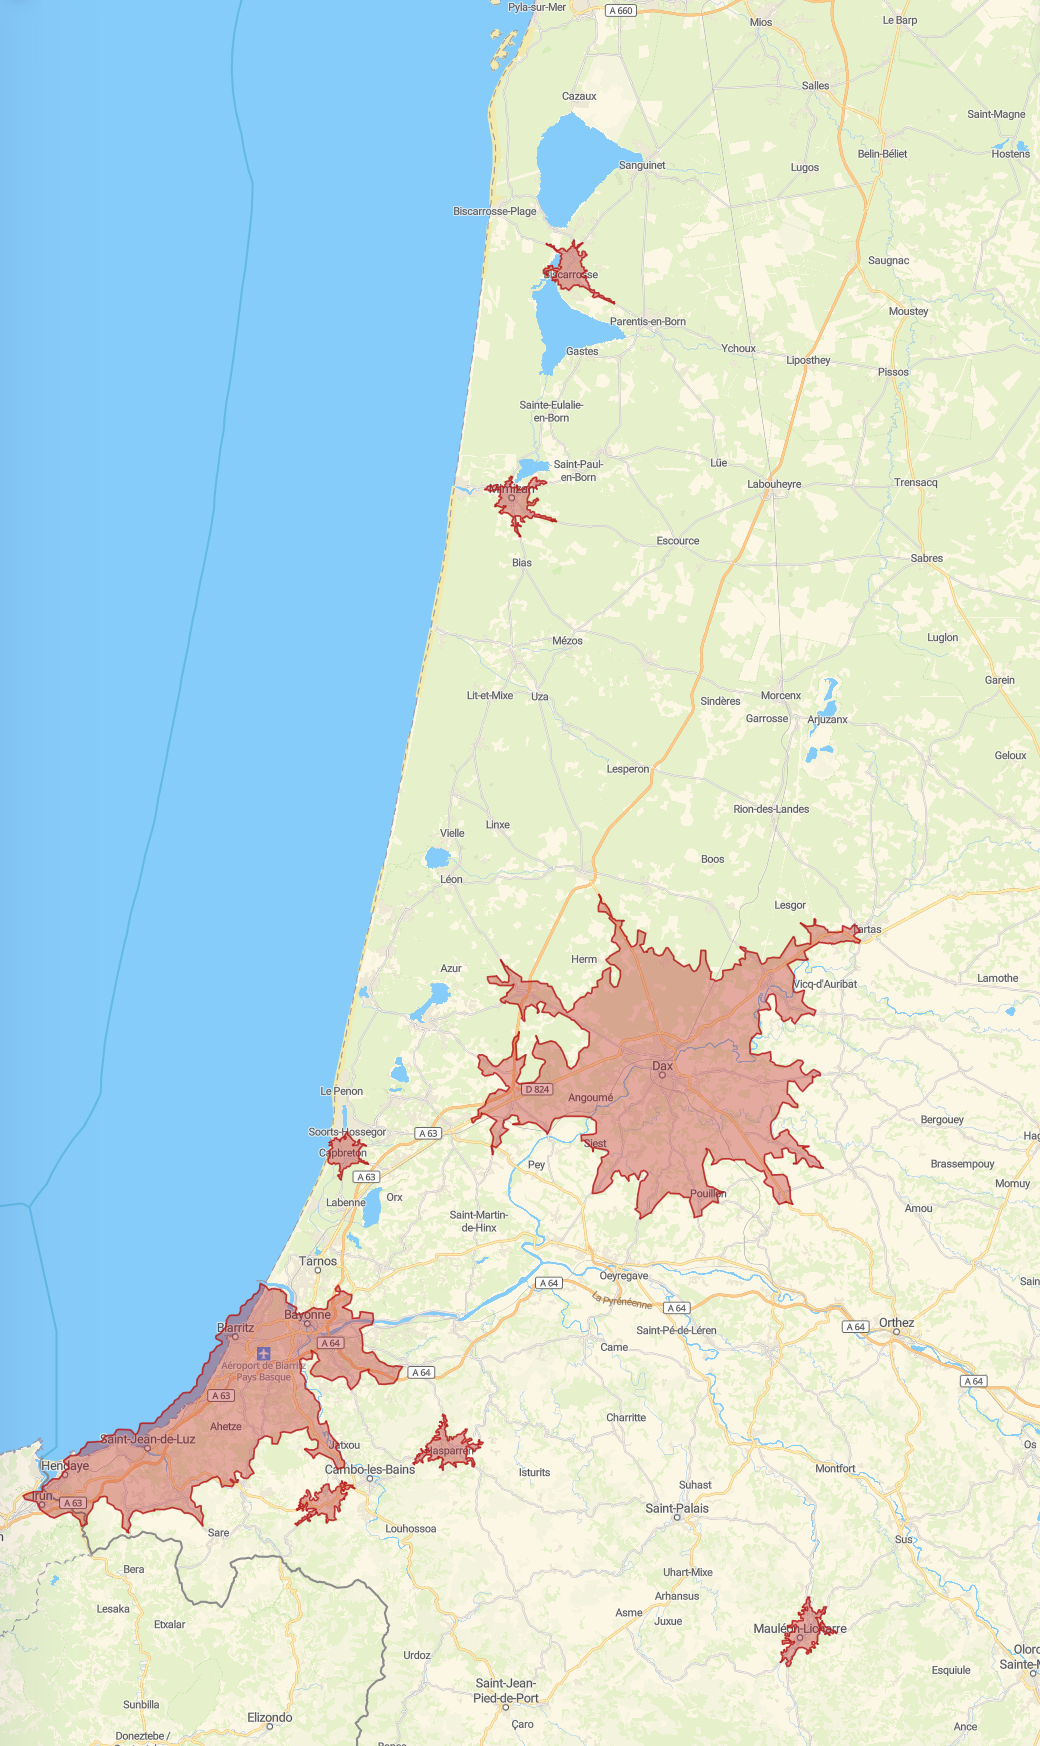
\includegraphics[width=\textwidth - \textwidth / 5]{zone_chalandise_aditu.png}
%     %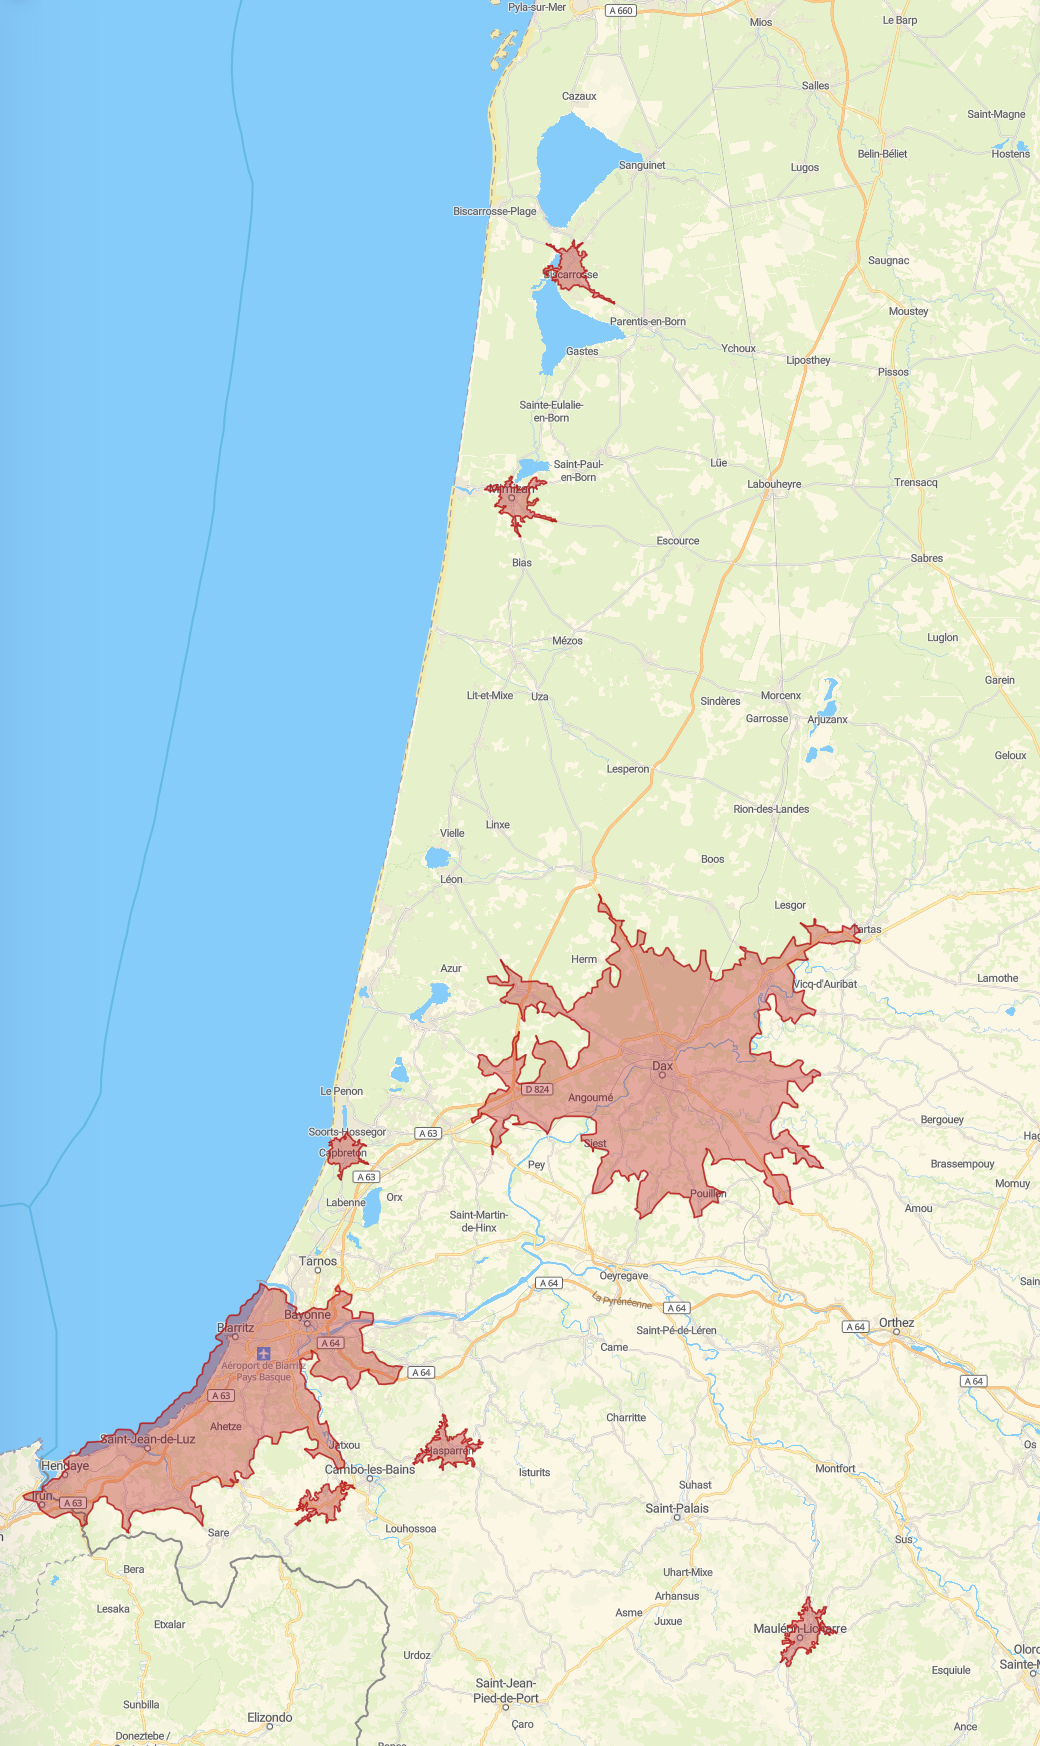
\includegraphics[scale=0.2]{zone_chalandise_aditu.png}
%     \figurename
%     \caption{Visualisation de la zone de chalandise d'ADITU, regroupée autour de ses datacenters à Bidart et à Dax}
%     \label{fig:zone_chalandise}
% \end{figure}

% \section{Cahier des charge Ticketing}

% % \begin{figure}[H]
% %     \centering
% %     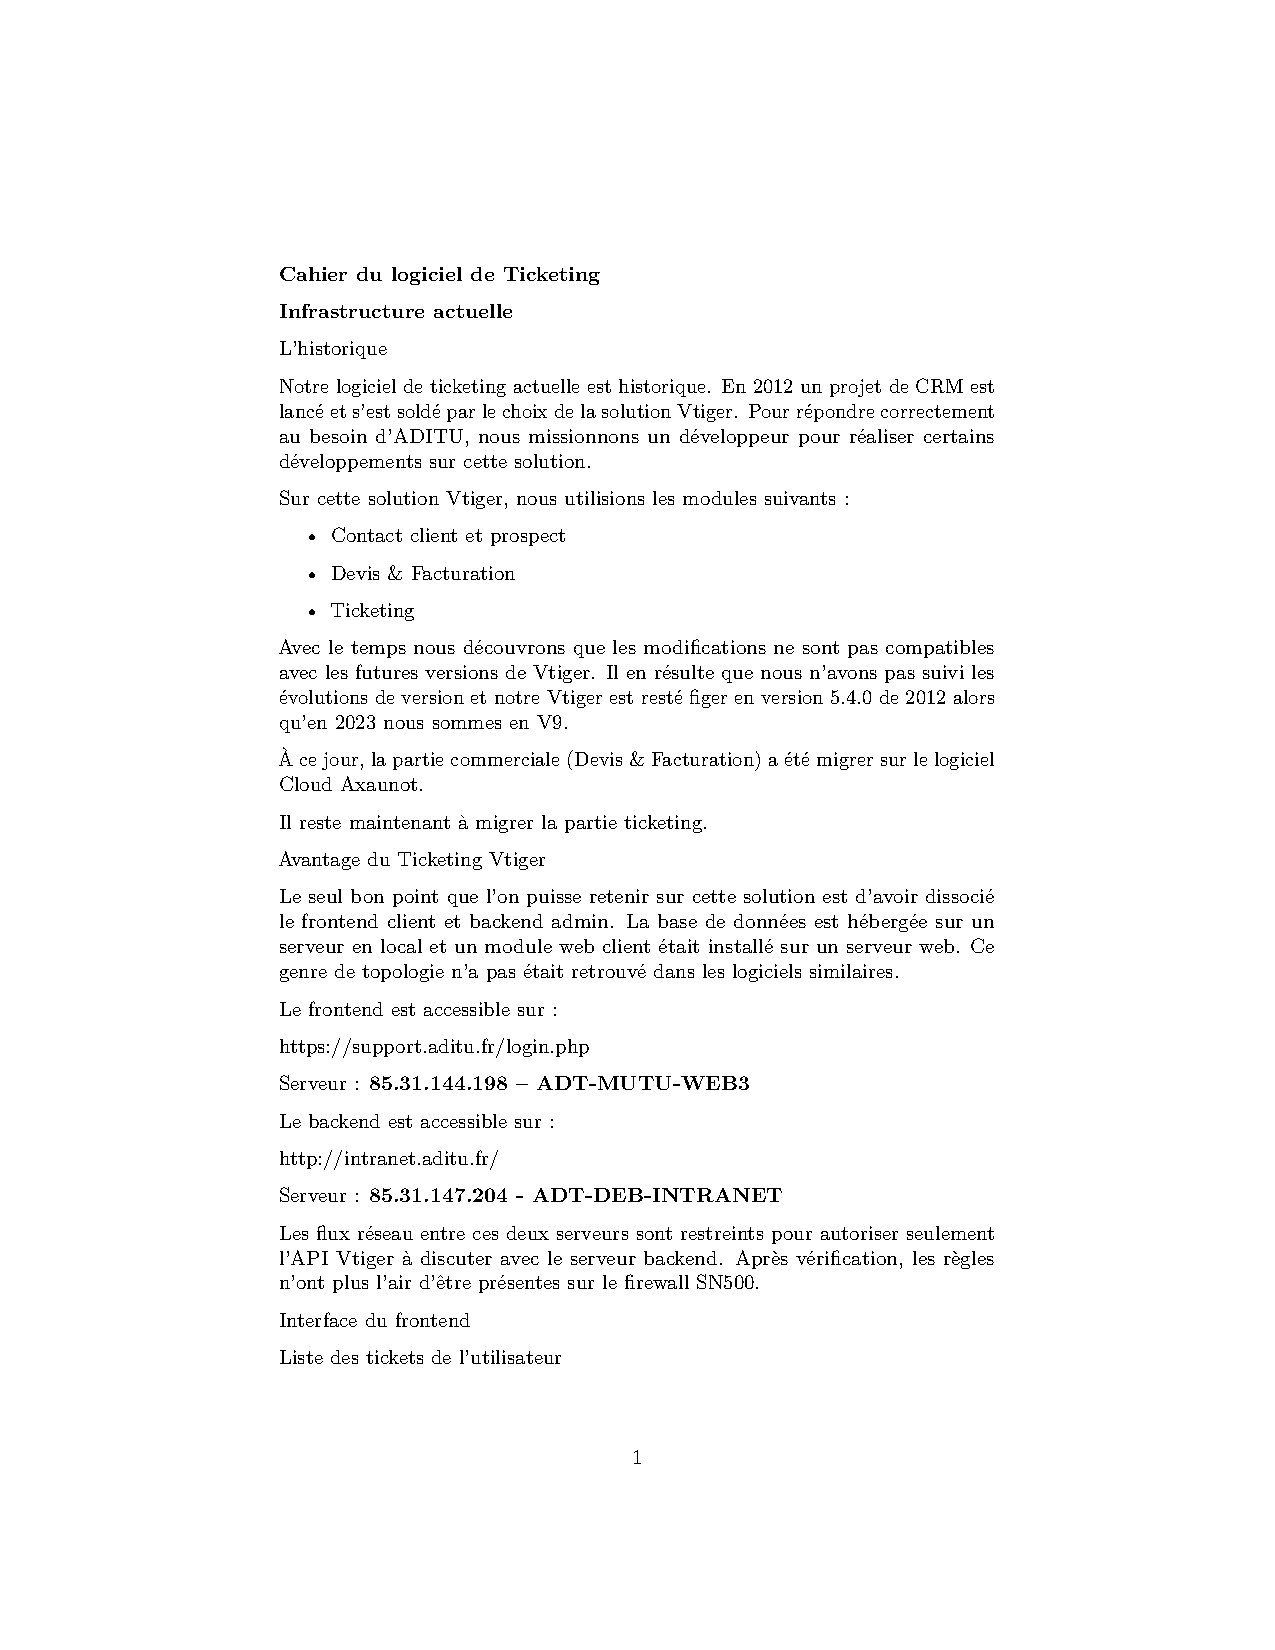
\includegraphics[width=\textwidth - \textwidth / 20]{CDC-Ticketing.pdf}
% %     \figurename
% %     \caption{Fiche de poste de notre alternance}
% %     \label{fig:poste}
% % \end{figure}

% \textbf{Cahier du logiciel de Ticketing}

% \textbf{Infrastructure actuelle}

% L'historique

% Notre logiciel de ticketing actuelle est historique. En 2012 un projet
% de CRM est lancé et s'est soldé par le choix de la solution Vtiger. Pour
% répondre correctement au besoin d'ADITU, nous missionnons un développeur
% pour réaliser certains développements sur cette solution.

% Sur cette solution Vtiger, nous utilisions les modules suivants~:

% \begin{itemize}
% \item
%   Contact client et prospect
% \item
%   Devis \& Facturation
% \item
%   Ticketing
% \end{itemize}

% Avec le temps nous découvrons que les modifications ne sont pas
% compatibles avec les futures versions de Vtiger. Il en résulte que nous
% n'avons pas suivi les évolutions de version et notre Vtiger est resté
% figer en version 5.4.0 de 2012 alors qu'en 2023 nous sommes en V9.

% À ce jour, la partie commerciale (Devis \& Facturation) a été migrer sur
% le logiciel Cloud Axaunot.

% Il reste maintenant à migrer la partie ticketing.

% Avantage du Ticketing Vtiger

% Le seul bon point que l'on puisse retenir sur cette solution est d'avoir
% dissocié le frontend client et backend admin. La base de données est
% hébergée sur un serveur en local et un module web client était installé
% sur un serveur web. Ce genre de topologie n'a pas était retrouvé dans
% les logiciels similaires.

% Le frontend est accessible sur~:

% \url{https://support.aditu.fr/login.php}

% Serveur~: \textbf{85.31.144.198 -- ADT-MUTU-WEB3}

% Le backend est accessible sur~:

% \url{http://intranet.aditu.fr/}

% Serveur~: \textbf{85.31.147.204 - ADT-DEB-INTRANET}

% Les flux réseau entre ces deux serveurs sont restreints pour autoriser
% seulement l'API Vtiger à discuter avec le serveur backend. Après
% vérification, les règles n'ont plus l'air d'être présentes sur le
% firewall SN500.

% Interface du frontend

% Liste des tickets de l'utilisateur

% 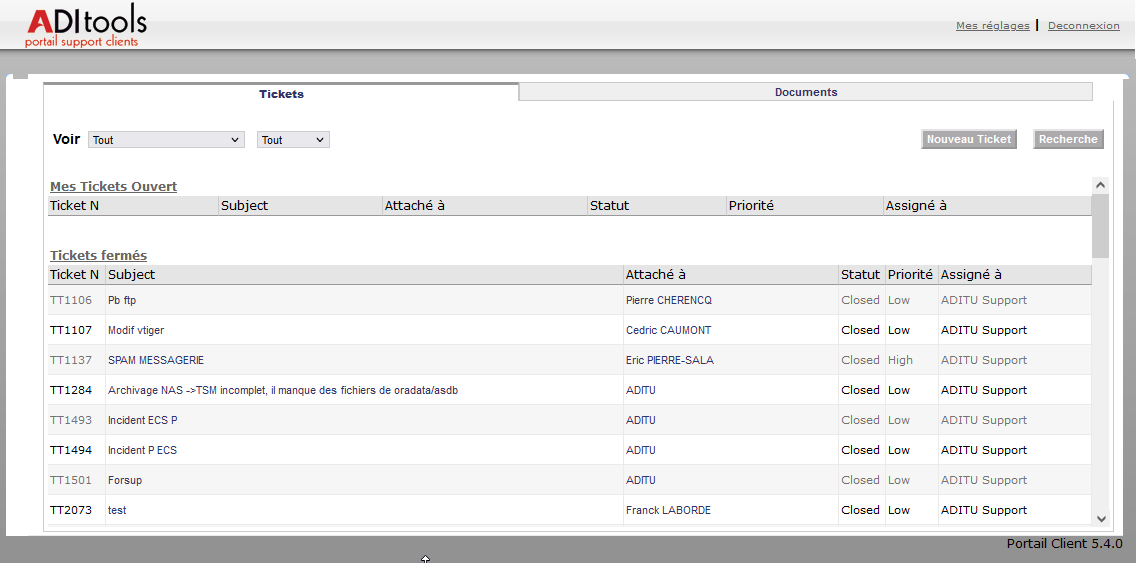
\includegraphics[width=6.3in,height=3.12222in]{image1.png}

% Création de tickets

% 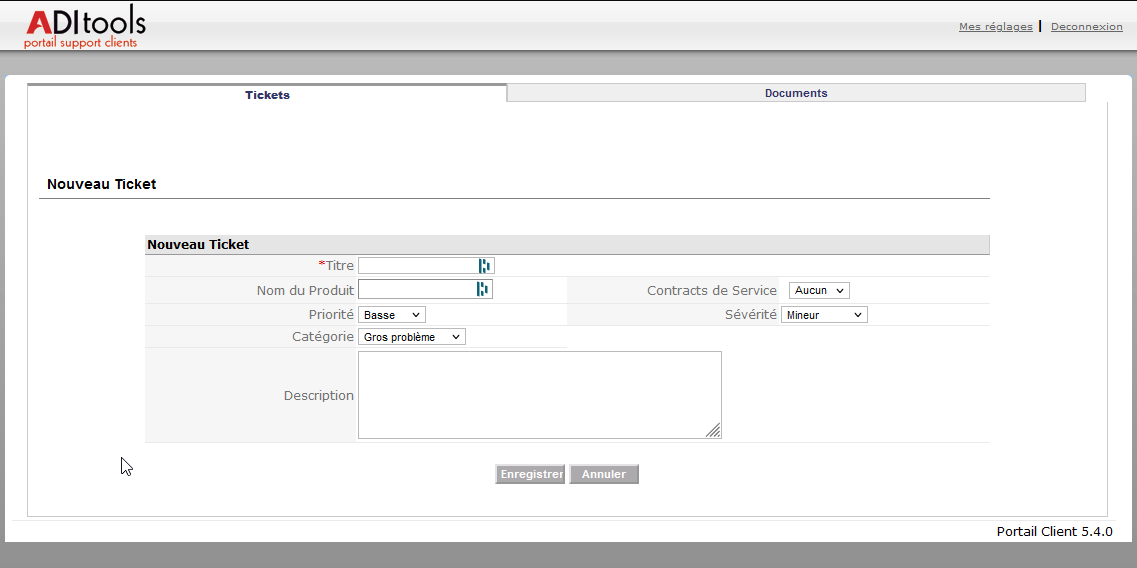
\includegraphics[width=6.3in,height=3.14722in]{image2.png}

% On peut constater que l'interface est plutôt minimaliste et
% vieillissante. Il manque certaines fonctions qui seront abordées plus
% bas.

% \textbf{Nouveau logiciel souhaité}

% Nous souhaitons migrer vers un nouveau logiciel de ticketing qui puisse
% intégrer les fonctionnalités ci-dessous~:

% Création d'incidents

% \begin{quote}
% La gestion des incidents permet de suivre et de résoudre les incidents
% signalés par les utilisateurs.
% \end{quote}

% Création de demandes de changement

% \begin{quote}
% Gestion des changements permet de planifier, suivre et gérer les
% modifications demandées par les utilisateurs.

% Exemple~: modification de ports sur le firewall, augmenter une boite aux
% lettres, etc.
% \end{quote}

% Création de tickets automatiquement

% \begin{quote}
% Cette fonctionnalité permet de planifier des interventions récurrentes
% sans les oublier. Exemple~: test de restauration
% \end{quote}

% Gestion des ressources

% \begin{quote}
% Pouvoir lié du matériel ou logiciel a un client et faire un suivi des
% modifications sur ce cette ressource.

% Exemple~: avoir le suivi des modifications comme celui qui est présent
% sur la page client du wiki.

% Intégrer du matériel lié à un fournisseur et gérer sa garantie. Exemple
% NAS ANANDA.

% Gérer les renouvellements~: des certificats

% Gérer les renouvellements~: des noms de domaines
% \end{quote}

% Inventaires

% \begin{quote}
% Lister l'ensemble des machines (connecteur OCS)
% \end{quote}

% Tableaux de bord et rapports

% Avoirs des stats et indicateurs sur ce qui nous prend le plus de temps
% dans le support.

% Ergonomique

% \begin{quote}
% Il faut que le logiciel soit intuitif et ergonomique. Que l'utilisateur
% ne soit pas rebuté par la complexité d'ouverture d'un ticket.
% \end{quote}

% Ouverture de ticket via email

% Fermeture de ticket automatique après un délai de non-réponse

% Personnalisation graphique

% \begin{quote}
% Nous souhaitons que l'application puisse se personnaliser aux couleurs
% de la société et d'y insérer le logo.
% \end{quote}

% Récupération des données ticketing vtiger

% \begin{quote}
% Seulement si cette récupération est facile. Ne pas perdre du temps sur
% cette récupération.
% \end{quote}

% Fonctions annexes

% Gestion des baies racks du datacenter


    % Pós Textuais
    % \nocite{*}
    % \include{pos-textuais/referencias}

\end{document}
